\section{İLETİM ORTAMLARI}
Temelde atmosfer ve kablo olmak üzere iki farklı iletim ortamı mevcuttur. Atmosferde RF (radyo frekans) dalgalarını kullanarak  iletişim gerçekleşir.
Kablolarda ise genellikle fiberoptik ve bakır kablo kullanılmaktadır.

\subsection{İKİ TELLİ BAKIR TELEFON HATTI }
Telefon iletişimini sağlamak için tasarlanmıştır. Temel bant ve geniş bant internet hizmeti verilmektedir.
Analog modülasyon teknikleriyle en fazla 56 k b/s'lik band genişliği sağlar. xDSL teknolojileriyle 25 Mb/s'lik bant genişliğine ulaşmaktadır.  
\begin{figure}[!ht]
    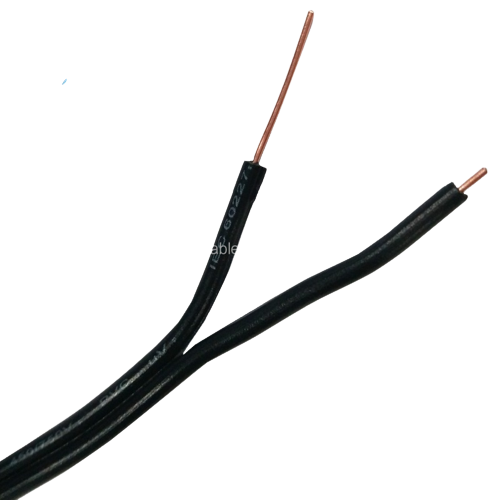
\includegraphics{images/ikitellibakirkablo}
   \caption{İki telli Bakir Kablo}
    \label{fig:iki_telli_bakir_kablo}
 \end{figure}

 \subsection{KOAKSİYEL (COAXIAL) KABLO}
 Genellikle elektriksel gürültünün yoğun olduğu şartlarda kullanılırdı.Yalıtkan bir tüpün içerisinde  giden bir tel ve tüpün dışına sarılmış kafes şeklinde teller vardır.
 Yerel ağlarda (LAN) 180m'de(max) 10M b/s bant genişliği sağlar. Bu kullanımı 10 Base 2 olarak bilinir. Daha sonra 500 m mesafede çalıştırılacak hale getirilir. 10 Base 2 ismiyle standartlaştırılmıştır. 50 ohm'luk direnç değeri vardır.
 BNC tarzında konnektörler kullanılır. Günümüzde LAN'da hiç kullanılmamaktadır. Sebebi hem 10 Mb/s hızının çok düşük olması, hem de UTP kablolar kadar ekonomik ve işlevsel olmamasıdır.
 Bilgisayar ağlarında doğrusal (bus) topolojilerde kullanılmıştır. 
 
  \begin{figure}[!ht]
     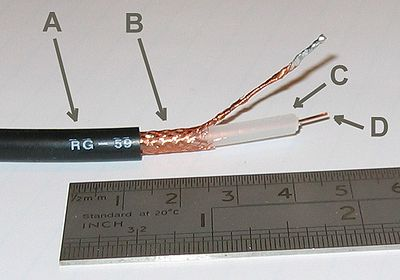
\includegraphics{images/400px-RG-59}
    \caption{Koaksiyel Kablo}
     \label{fig:kooksiyel_kablo}
  \end{figure}


 \section*{AĞ TOPOLOJİLERİ }
\begin{figure}[!ht]
    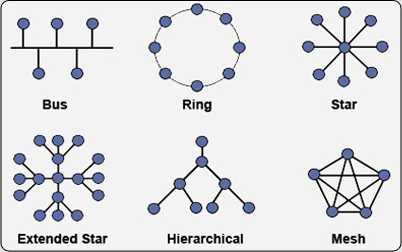
\includegraphics{images/62_ağ_topolojisi}
   \caption{Topolojiler}
    \label{fig:topolojiler}
 \end{figure}
 % bu kısım notlarda yok topoloji nedir kısmını ben ekledim.
Ağ topolojileri nedir sorusunun en net cevabı, "bir ağı oluşturan cihazların fiziksel ve mantıksal yerleşimidir". Network Topology (Ağ Topolojisi) Yerel Ağ Alanı (LAN) içerisinde bulunan bilgisayarların fiziksel ve mantıksal yerleşimini ifade eder. Fiziksel Topoloji ağ içerisinde bulunan tüm cihazların birbirlerine nasıl bağlanacağını ve bağlantı için ne tür kablo kullanacağını belirtirken Mantıksal Topoloji bu cihazların nasıl haberleşeceğini belirtir ve bu cihazları ortak bir protokol altında birleştirir. Kullanılmak istenen Ağ Teknolojisine göre farklı ağ topolojileri kullanılmaktadır.
Fiziksel Topolojinin 6 farklı çeşidi vardır. Bunlar Bus(Yol), Ring(Halka), Yıldız(Star), Ext Star(Gelişmiş Yıldız), Mesh(Örgü) ve Tree(Ağaç) topolojileridir. Broadcast(Yayın) ve Token Passing(İz) mantıksal topolojilere birer örnektir.

\subsection*{DOĞRUSAL (BUS) TOPOLOJİ}
Doğrusal bir hat üzerinde bilgisayarların T konnektörlerle bağlanması şeklinde kurulur. Hattın her iki ucunda sonlandırıcı kullanmak zorunludur. Koaksiyel kablo kullanılır. Ağın herhangi  bir noktasında arıza olması durumunda ağın tamamı çöker.Ağdaki veri trafiği tüm uçlara gider. Herkes herkesin trafiğini görebilir. Bu yüzden çok fazla \textbf{çakışma (colision)} olur.
\begin{figure}[!ht]
    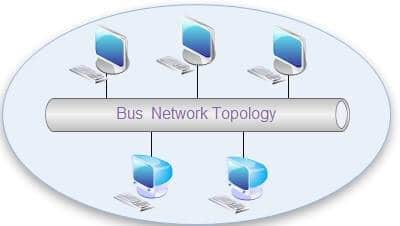
\includegraphics{images/bus-topolojisi}
   \caption{Bus Topolojisi}
   \label{fig:bustopolojisi}
 \end{figure}

\subsection*{HALKA (RING) TOPOLOJİ}
Doğrusal topolojiye benzer. Sonlandırıcı kullanılmaz. Hattın iki ucu birleşiktir. Hatta sanal  bir jeton dolaşır(token).Jeton sırası gelen bilgisayar, jeton boş ise göndereceği veriyi hatta yerleştirir.
Bilgisayarlar sırayla  veri gönderdiklerinden çakışma daha azdır.Günümüzde hiç kullanılmamaktadır. Herkes herkesin verisini kullanabilmektedir.
%bu fotoğraf en alta geçiyor düzeltilecek
\begin{figure}[!ht]
    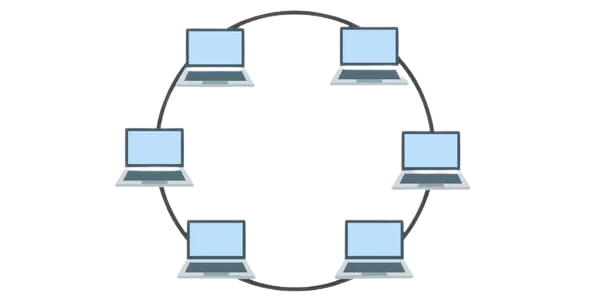
\includegraphics{images/ring-topology-removebg-preview}
    \caption{Halka-Ring Topolojisi}
   \label{fig:halka_topolojisi}
  \end{figure}


\subsection*{YILDIZ (STAR) TOPOLOJİ}
Merkezde dağıtıcı bir cihaz olur. Buradan tüm bilgisayarlara birer kablo gider. Ağın bir noktasındaki arıza sadece ilgili bilgisayarın ağ bağlantısına zarar verir. Genellikle \textbf(bükümlü çift (twisted pair,xtp)) kullanılır. Trafiğin herkese mi gönderileceği ya da sadece ilgili uca mı gideceği dağıtıcıya bağlıdır. Dağıtıcının  performansı ve kabiliyeti ağı doğrudan  etkiler. Günümüzde en yaygın topolojidir.
%YERİ DÜZELTİLECEK
\begin{figure}[!ht]
    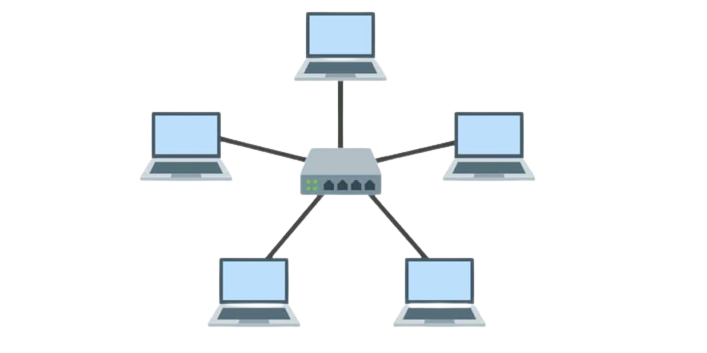
\includegraphics{images/star-Topology-1024x512-removebg-preview}
    \caption{Yildiz-StarTopolojisi}
   \label{fig:yildiz_topolojisi}
  \end{figure}

\subsection*{ÖRGÜ (MESH)TOPOLOJİ}
%YERİ DÜZELTİLECEK
\begin{figure}[!ht]
 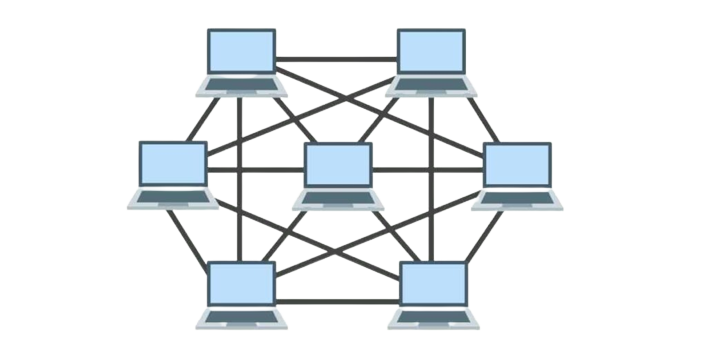
\includegraphics{images/mesh-topology-1-1024x512-removebg-preview}
    \caption{Örgü-Mesh Topolojisi}
   \label{fig:Orgu_mesh_topolojisi}
  \end{figure}
Uçları arasında birden fazla rota üzerinde haberleşme imkanı olan yapılardır.
Günümüzde genellikle farklı yıldız ağlar arasında yedekleme amacı olarak kullanılır.

\subsection{BÜKÜMLÜ ÇİFT KABLO}
  İçerisinde 4 çift bakır kablo bulunur.Kabloların birbirleri üzerindeki direnç elektromanyetik etkisini azaltmak için ikişerli olarak sarılı durumundadırlar.
  Örneğin; UTP,CAT5,Ethernet Kablosu 
  \begin{figure}[!ht]
   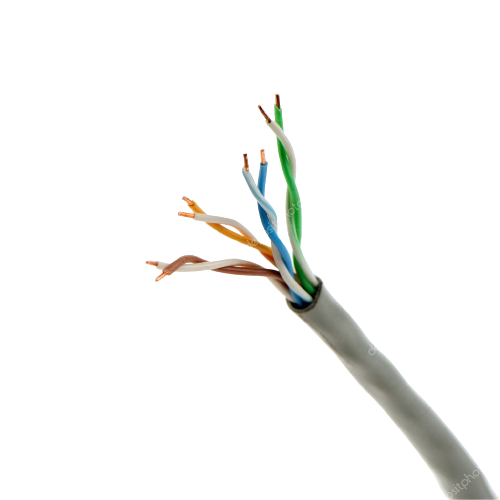
\includegraphics{images/bukumlukablo}
   \caption{Bükümlü çift kablodan bir kesit}
 \label{fig:Bukumlu_cift_kablo}
 \end{figure}

\subsubsection{UTP (UNSHILDED TWISTED PAIR) Korumasız Bükümlü Çift} 
8 iletkenin her biri ince bir yalıtkan ile kaplanmıştır. En dışında tamamını kaplayan bir yalıtkan vardır.
\subsubsection{STP(SHİLDED TWİSTED PAİR)} 
Her çiftin altında koruma (topraklama ) vardır.
\subsubsection{FTP(FOİLED TWİSTED PAİR )} 
4 çiftin tamamının etrafında folyo koruma vardır.
\subsubsection {S/FTP }
İkisinin de özelliğini taşımaktadır.
    
\subsection{FREKANSLARINA GÖRE BÜKÜMLÜ ÇİFT KABLO}
\textbf{CAT:}\\
\textbf{CAT1-CAT3} \\
Telefon hatlarında bulunur.\\
\textbf{CAT5} \\
En yaygın kullanılan ağ kablosudur. Azami 100m mesafe ve 10Mb/s destekler.\\
\textbf{CAT6} \\
100 m mesafede 1G b/s destekler.\\
\textit{10 BASE T} Ethernet(Eth)\\
\textit{100 BASE T} Fast Ethernet(Fa,Fe)\\
\textit{1000 BASE T} Gigabit Ethernet(G,GE)\\
Bükümlü çift CAT5 VE CAT6 Kabloları  sonlandırmak için RJ-45 adı verilen konnektörler kullanılır.
Bu kablolar iki farklı iki şekilde sonlandırılabilir.\textbf{568-A,568-B}\\
Kablonun iki ucunun aynı standartlarla sonlandırılmasına \textbf{düz (Straight kablo)} denir. İki ucunda iki farklı standartta sonlandırılma yapılırsa \textbf{çapraz(cross-over)kablo } adı verilir.
\subsection{ÇAPRAZ VE DÜZ KABLO}
Düz kablo, bir bilgisayarı yönlendirici gibi bir ağ hub'ına bağlamak için yerel alan ağlarında kullanılan bir tür bükümlü çift kablodur. Bu tür kablolara bazen yama kablosu da denir ve bir veya daha fazla bilgisayarın kablosuz bir sinyal yoluyla bir yönlendiriciye eriştiği kablosuz bağlantılara bir alternatiftir. Aynı türden iki cihazı bağlamak için genellikle bir çapraz kablo kullanılır. Düz kablo ve çapraz kablo tasarımları aynı standartların ve kuralların çoğunu kullanır.

\begin{figure}[!ht]
  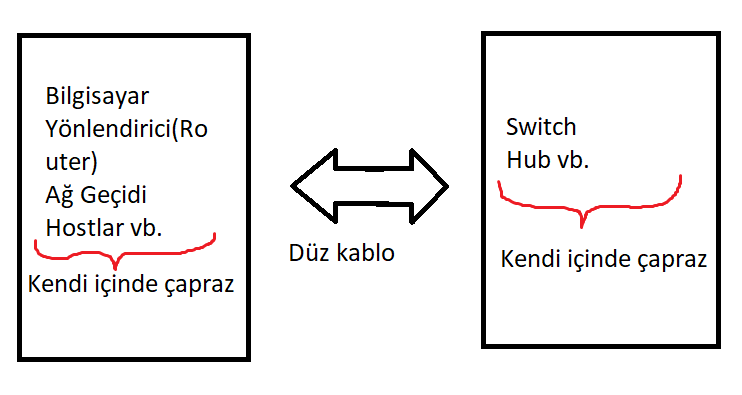
\includegraphics{images/caprazduzz}
 \caption{kablolar}
 \label{fig:caprazduz_kablo}
\end{figure}

Yeni ağ cihazlarının tamamı MDI/MDIX adı verilen teknoloji sayesinde karşıdaki cihazın ne tarz bir cihaz olduğunu anlar ve hangi iletkenin ne amaçla kullanılacağını buna göre  düzenler. Diğerleri enerji göndermek için kullanılır.

\begin{figure}[!ht]
  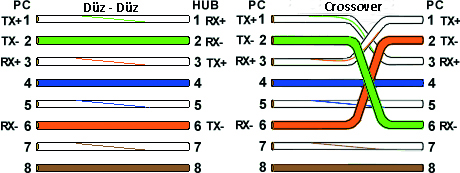
\includegraphics{images/ethcable}
 \caption{kablolar-örnek}
 \label{fig:caprazduz_kablo_ornek_gosterim}
\end{figure}
\section*{FİBER OPTİK KABLOLAR}